%\documentclass[referee,usenatbib]{mn2e}
\documentclass[useAMS,usenatbib, a4paper]{mn2e}

\usepackage{natbib}
\usepackage{graphicx}
\usepackage{url}
\usepackage[utf8]{inputenc}
\usepackage{fancyref}
\usepackage[T1]{fontenc}
\usepackage{array}
\usepackage{rotating}
\usepackage{units}
\usepackage{textcomp}
\usepackage{amsmath}
\usepackage{amsbsy}
\usepackage{amstext}
\usepackage[backref,breaklinks,colorlinks,citecolor=blue]{hyperref}

\newcommand{\msun}{\mbox{$\,{\rm M}_\odot$}}


\title[Gaia Challenge - Palomar 5]{The Gaia Challenge - recovering the galactic potential using a Palomar
5-like stream}

\author[K\"upper et al.]
{Andreas H.W. K\"{u}pper$^{1}$\thanks{
E-mail: \mbox{akuepper@astro.columbia.edu} (AK);
 \mbox{ana.bonaca@yale.edu} (AB);}
, Ana Bonaca$^{2}$, Nathan Deg$^{3}$, and so many more\\
$^{1}$Astronomy Department, Columbia University, 550 West 120th Street, New York City, NY 10027, USA\\
$^{2}$Department of Astronomy, Yale University, New Haven, CT 06511, USA\\
$^{3}$Wherever he may be\\
}

\begin{document}

%\date{Accepted 1988 December 15. Received 1988 December 14; in original form 1988 October 11}

%\pagerange{\pageref{firstpage}--\pageref{lastpage}} \pubyear{2002}

\maketitle

\label{firstpage}

\begin{abstract}
Kick-ass abstract
\end{abstract}




\begin{keywords}
globular clusters --- galactic dynamics
\end{keywords}

\bibliographystyle{mnras}



\section{Introduction}
Very introductory text.



\section{The Workshops}
Very interesting text about the Gaia Challenge workshops.



\section{The Palomar 5 Challenge}
This is a very interesting text about the Challenge.

We ran a direct $N$-body simulation of a Palomar 5-like globular cluster, which dissolved in a static background potential (see below). The model initially consisted of 65,356 particles and was evolved for 4\,Gyr using the publicly available code \textsc{Nbody6}. 

The Challenge can be found on the wiki page of the Gaia Challenge workshop\footnote{http://astrowiki.ph.surrey.ac.uk/dokuwiki/doku.php}, and we invite everybody to download the Challenge and contribute. The columns are described in the header of the file. They give Cartesian coordinates and observables for positions and velocities of all particles. All numbers are either in pc and km/s, or degree and mas/yr, respectively. 

The Cartesian coordinates are given in the Galactic rest frame. The observables were derived assuming a solar Galactocentric distance of 8.33 kpc and a LSR motion of 239.5\,km/s \citep{Gillessen09}. In addition, the solar reflex motion was assumed to be $(11.1, 12.24, 7.25)$\,km/s \citep{Schonrich10}.  

The present-day position of Palomar\,5 is $RA = 229.022083$\,deg, $Dec = -0.111389$\,deg or $l = 0.852059$\,deg, $b = 45.859989$\,deg, respectively. The present-day Cartesian coordinates of the progenitor are 
\begin{eqnarray}
  x &=& 7816.082584 pc\\
  y &=& 240.023507 pc\\
  z &=& 16640.055966 pc\\
  vx &=& -37.456858 km/s\\
  vy &=& -151.794112 km/s\\
  vz &=& -21.609662 km/s
\end{eqnarray}

\begin{itemize}
  \item $M_{Pal5}(t=-4 Gyr) = 31090\,M_{\odot}$
  \item $M_{Pal5}(t=today) = 13150\,M_{\odot}$
  \item $d_{Sun} = 23190\,pc$
\end{itemize}



\subsection{The potential}

The functional form of the potential components is as follows:

Flattened NFW halo:

\begin{eqnarray}
  \Phi_{Halo}(R, z) &=& -\frac{GM}{\sqrt{R^2+\frac{z^2}{q_z^2}}}\ln\left(1+\frac{\sqrt{R^2+\frac{z^2}{q_z^2}}}{R_{Halo}} \right)\\
  M_{Halo} &=& 1.81194\times 10^{12}\msun\\
  R_{Halo} &=& 32260\,pc\\
  q_z &=& 0.8140
\end{eqnarray}

Jaffe bulge:

\begin{eqnarray}
  \Phi_{Bulge} &=& -\frac{GM_{Bulge}}{b_{bulge}}\ln{\frac{R}{R+b_{bulge}}}\\
  M_{Bulge} &=& 3.4\times 10^{10}\msun\\
  b_{Bulge} &=& 700.0\,\mbox{pc}
\end{eqnarray}

Miyamoto-Nagai disk:
\begin{eqnarray}
  \Phi_{Disk} &=& -\frac{GM_{Disk}}{\sqrt{R^2+\left(a_{Disk}+\sqrt{z^2+b_{Disk}^2}\right)^2}}\\
  M_{Disk} &=& 1.0\times 10^{11}\,M_{\odot}\\
  a_{Disk} &=& 6500\,pc\\
  b_{Disk} &=& 260\,pc
\end{eqnarray}

\begin{itemize}
  \item $V_C(R_{Sun}) = 249.01\,km/s$
  \item $V_C(R_{Pal5}) = 247.84\,km/s$
  \item $V_C(R_{Halo}) = 251.99\,km/s$
  \item $a(R_{Sun}, 0, 0) = 7.95\,pc/Myr^2$
  \item $a(R_{Pal5}) = a(7816 pc, 240 pc, 16640 pc) = 3.51\,pc/Myr^2$
  \item $a(R_{Halo}, 0, 0) = 2.06\,pc/Myr^2$
\end{itemize}





\section{The Methods}
Quite interesting text about the methods.

\subsection{Nathan Deg}
Nathan's method is described in \citet{Deg13}.



\section{Results}
Many interesting results.

\subsection{Ana Bonaca}
For Ana's results see Fig.~\ref{plot_ana_results}
\begin{figure*}
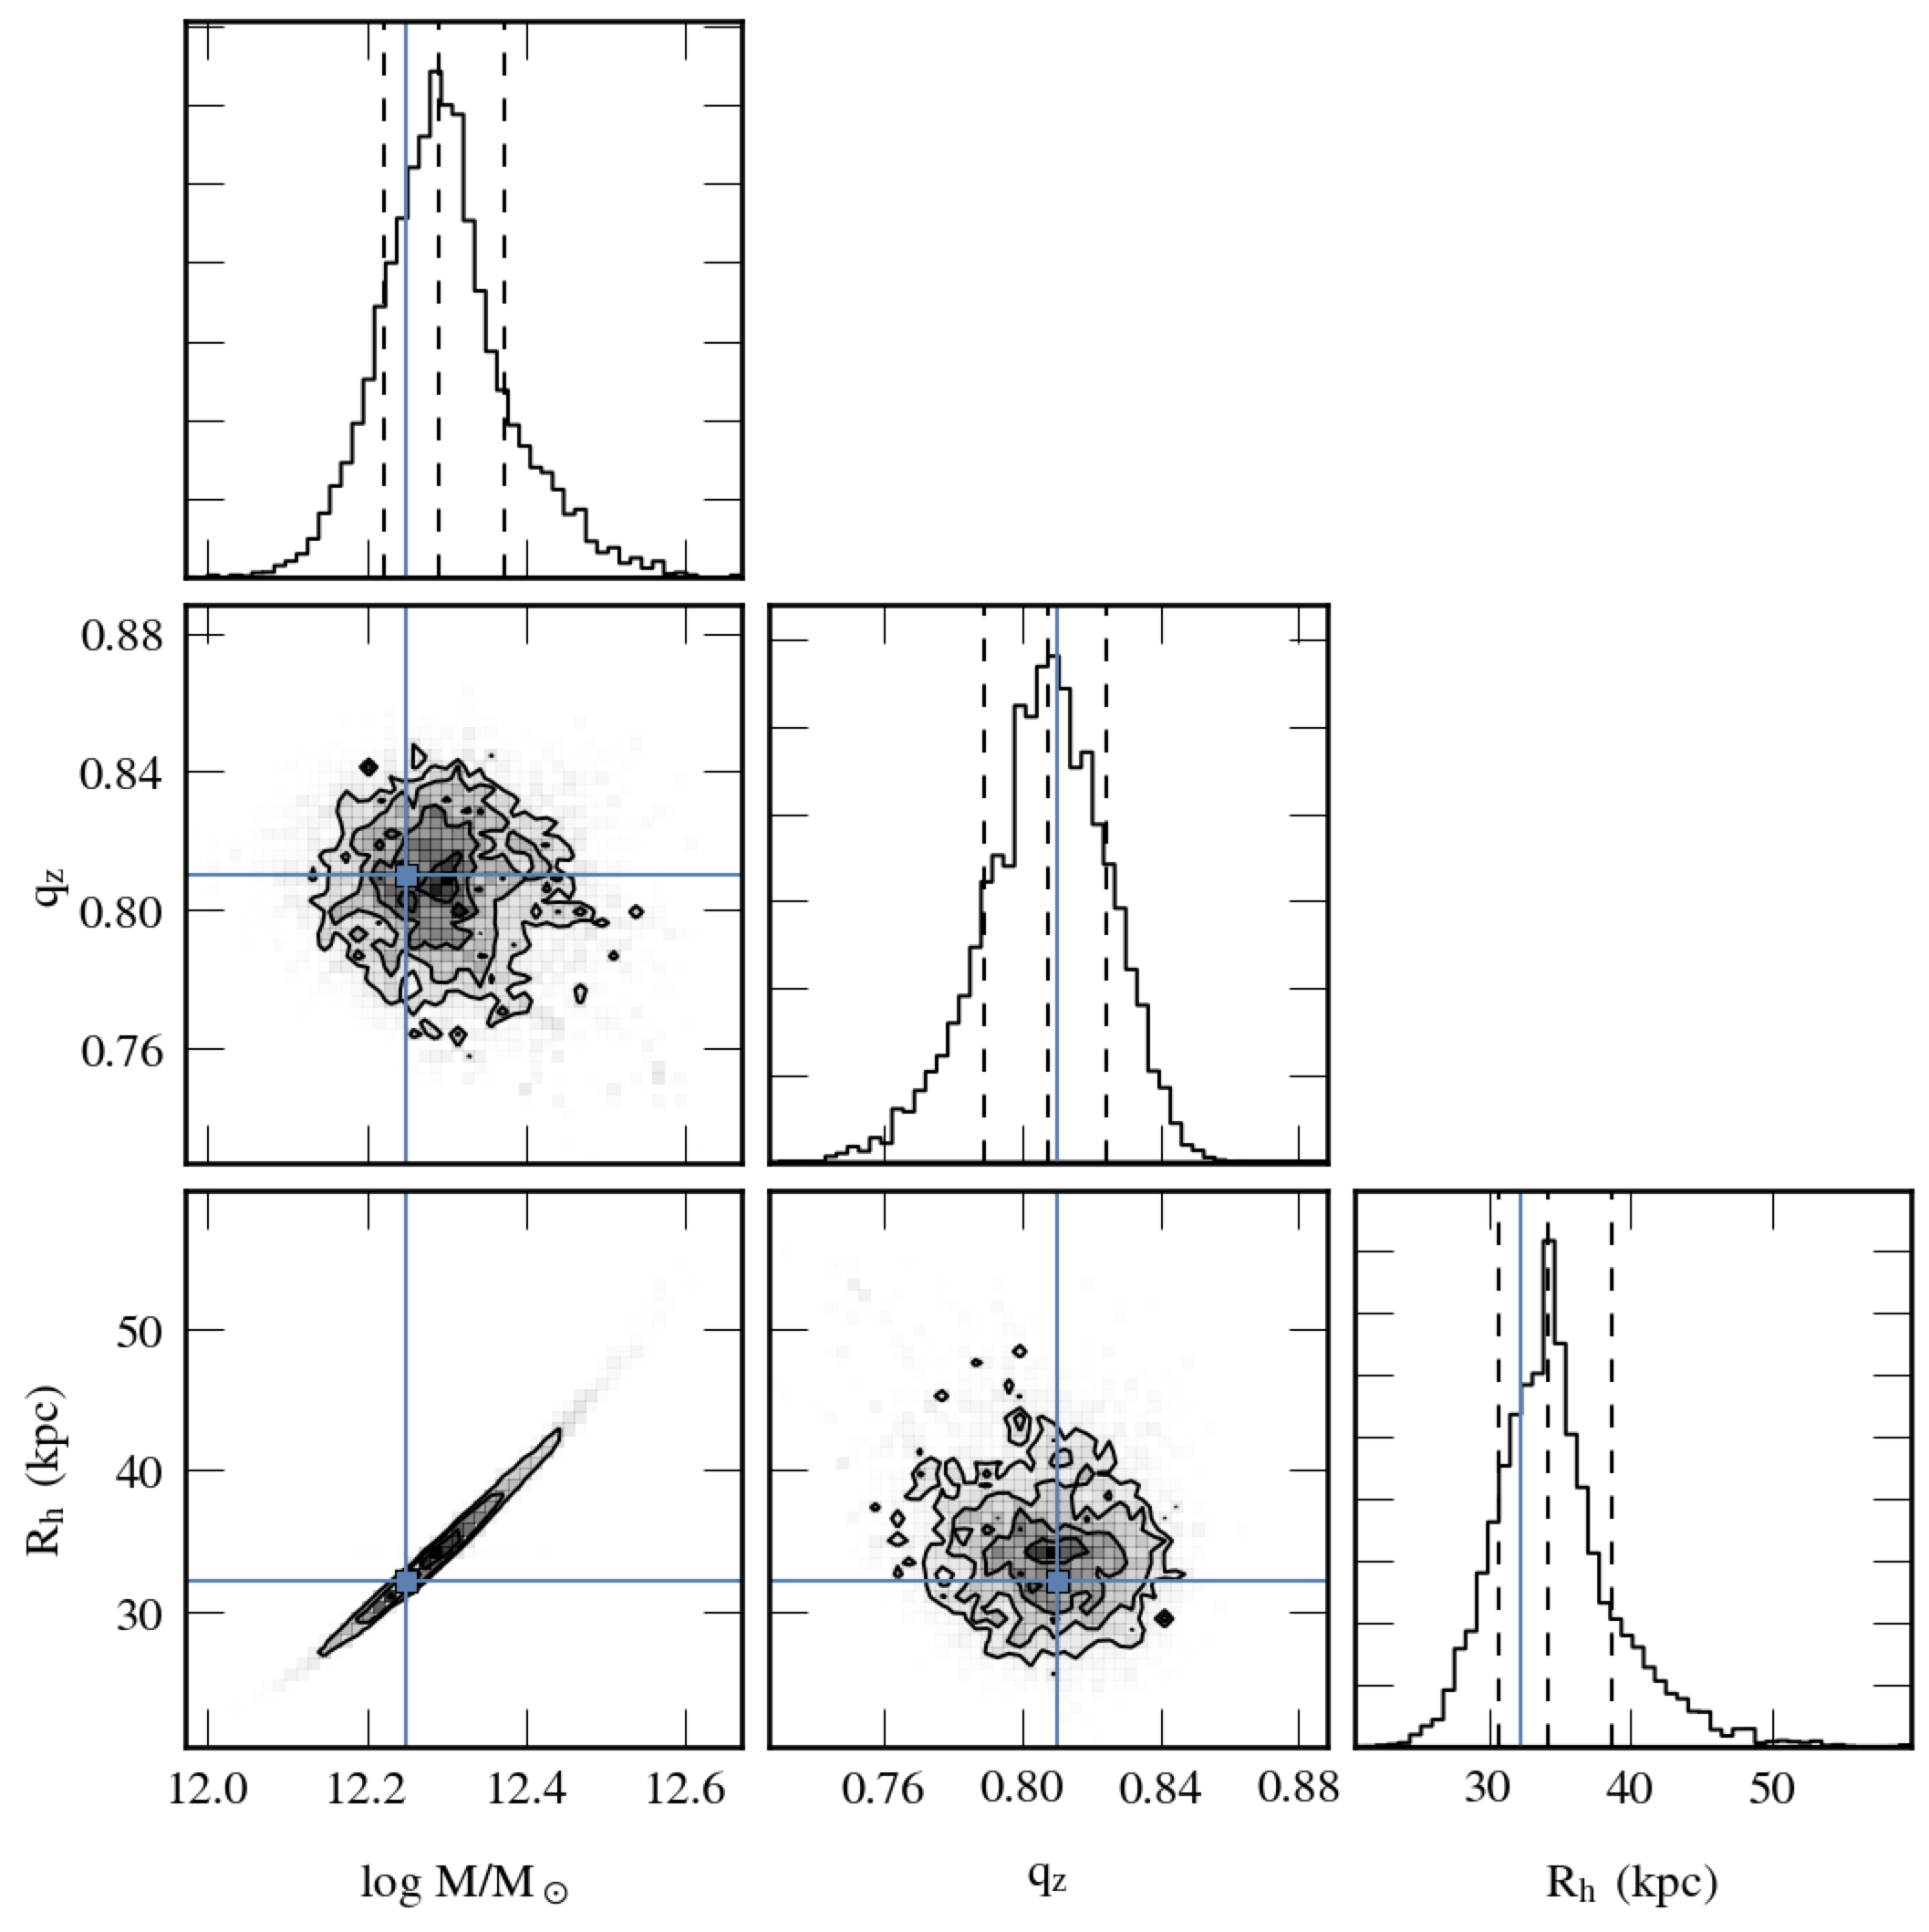
\includegraphics[width=168mm]{ana_results.png}
  \caption{...}
  \label{plot_ana_results}
\end{figure*}


\subsection{Nathan Deg}
This subsection is dedicated to Nathan.




\section{Conclusions}
Oh man, all these conclusions!


\section*{Acknowledgements}
\input{acknowledgements.tex}

\begin{thebibliography}{99}
\bibitem[\protect\citeauthoryear{Deg \& Widrow}{2013}]{Deg13} 
Deg N., Widrow L., 2013, MNRAS, 428, 912 

\bibitem[\protect\citeauthoryear{Gillessen et al.}{2009}]{Gillessen09} 
Gillessen S., Eisenhauer F., Trippe S., Alexander T., Genzel R., Martins F., Ott T., 2009, ApJ, 692, 1075 

\bibitem[\protect\citeauthoryear{Sch{\"o}nrich, Binney, \& Dehnen}{2010}]{Schonrich10} 
Sch{\"o}nrich R., Binney J., Dehnen W., 2010, MNRAS, 403, 1829 


\end{thebibliography}



\bsp \label{lastpage} \end{document}

